\documentclass{article}
\usepackage{tikz, comment}
\usepackage{pifont}
\usepackage{fontspec}
\usetikzlibrary{arrows, decorations.markings, decorations.pathreplacing}
\begin{comment}
:Title: Not defined yet
:Tags: intersection;figure;curves;angles
:Author: Prof.Hu Ji-shan, HKUST
:Slug: No name yet

Description Here.........
\end{comment}
\begin{document}\centering

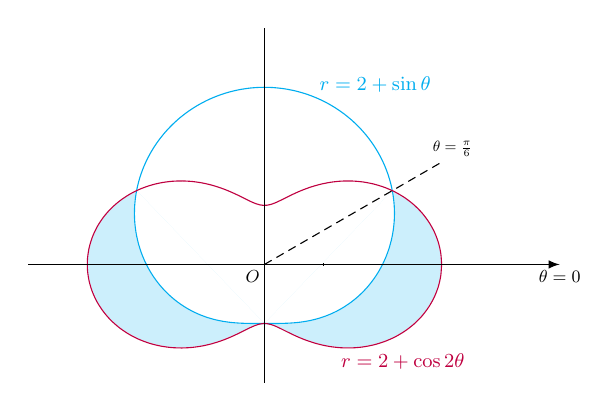
\begin{tikzpicture}[>=latex,xscale=.5*1.5, yscale=.5*1.5][font=\sf\small]

%\draw[xstep=1cm,ystep=1cm,color=gray!80] (0, -1) grid (8, 8);

\draw[white, fill=cyan!20, samples=100, smooth, domain=-pi/2:pi/6, variable=\t]
plot ({(2+cos(2*\t r))*cos(\t r)}, {(2+cos(2*\t r))*sin(\t r)});

\draw[white, fill=white, samples=100, smooth, domain=-pi/2:pi/6, variable=\t]
plot ({(2+sin(\t r))*cos(\t r)}, {(2+sin(\t r))*sin(\t r)});

\draw[white, fill=cyan!20, samples=100, smooth, domain=5*pi/6:3*pi/2, variable=\t]
plot ({(2+cos(2*\t r))*cos(\t r)}, {(2+cos(2*\t r))*sin(\t r)});

\draw[white, fill=white, samples=100, smooth, domain=5*pi/6:3*pi/2, variable=\t]
plot ({(2+sin(\t r))*cos(\t r)}, {(2+sin(\t r))*sin(\t r)});

\draw[cyan, samples=100, smooth, domain=0:2*pi, variable=\t]
plot ({(2+sin(\t r))*cos(\t r)}, {(2+sin(\t r))*sin(\t r)});

\draw[purple, samples=100, smooth, domain=0:2*pi, variable=\t]
plot ({(2+cos(2*\t r))*cos(\t r)}, {(2+cos(2*\t r))*sin(\t r)});

\node[purple, xshift=50, yshift=-35, scale=0.8] at (0,0) {$r=2 + \cos 2\theta$};
\node[cyan, xshift=40, yshift=65, scale=0.8] at (0,0) {$r=2+\sin\theta$};

\draw[densely dashed, samples=100, smooth, domain=0:3, variable=\x]
plot ({\x}, {tan((pi/6) r)*(\x)})node[above, xshift=4, scale=0.6] {$\theta = \frac{\pi}{6}$};

\foreach \x in {1}
\draw (\x,2pt/3) -- (\x,-2pt/3)
node[anchor=north] {}%{\tiny$\x$}
;
\foreach \x in {}
\draw (\x,2pt/3) -- (\x,-2pt/3)
node[anchor=south] {\tiny$\x$}
;
\foreach \y in {}
\draw (-2pt/3,\y) -- (2pt/3,\y)
node[anchor=east] {}%{\tiny $\y$}
;

\draw[->] (-4, 0) -- (5, 0)node[below, scale=0.7] {$\theta=0$};
\draw[] (0, -2) -- (0, 4);

\node[scale=0.7] at (-0.3/1.5, -0.3/1.5) {$O$};

\end{tikzpicture}
\end{document}